%%%%%%%%%%%%%%%%%%%%%%%%%%%%%%%%%%%%%%%%%%%%%%%%%%%%%%%%%%%%%%%%%%%%%%%%%%%%%%%%
%2345678901234567890123456789012345678901234567890123456789012345678901234567890
%        1         2         3         4         5         6         7         8

\documentclass[letterpaper, 10 pt, conference]{ieeeconf}  % Comment this line out if you need a4paper

%\documentclass[a4paper, 10pt, conference]{ieeeconf}      % Use this line for a4 paper

\IEEEoverridecommandlockouts                              % This command is only needed if 
                                                          % you want to use the \thanks command

\overrideIEEEmargins                                      % Needed to meet printer requirements.

%In case you encounter the following error:
%Error 1010 The PDF file may be corrupt (unable to open PDF file) OR
%Error 1000 An error occurred while parsing a contents stream. Unable to analyze the PDF file.
%This is a known problem with pdfLaTeX conversion filter. The file cannot be opened with acrobat reader
%Please use one of the alternatives below to circumvent this error by uncommenting one or the other
%\pdfobjcompresslevel=0
%\pdfminorversion=4

% See the \addtolength command later in the file to balance the column lengths
% on the last page of the document

% The following packages can be found on http:\\www.ctan.org
\usepackage{graphics} % for pdf, bitmapped graphics files
\usepackage{epsfig} % for postscript graphics files
\usepackage{mathptmx} % assumes new font selection scheme installed
\usepackage{times} % assumes new font selection scheme installed
\usepackage{amsmath} % assumes amsmath package installed
\usepackage{amssymb}  % assumes amsmath package installed
\usepackage{mathtools}
\usepackage{relsize}
\usepackage{tikz}
\graphicspath{{./Drawings/}} 
\newcommand{\notimplies}{%
	\mathrel{{\ooalign{\hidewidth$\not\phantom{=}$\hidewidth\cr$\implies$}}}}
\usepackage[margin=0.8cm]{caption}
\newcommand{\norm}[1]{\left\lVert#1\right\rVert}
\usepackage{pgfplots}
\pgfplotsset{compat=newest}
\pgfplotsset{plot coordinates/math parser=false}
\newlength\figureheight
\newlength\figurewidth 
\usepackage{adjustbox}
\usepackage{indentfirst}


\setlength{\parindent}{15pt} % Default is 15pt.


\title{\LARGE \bf
Robust data-driven predictive control
}


\author{Sampath Kumar Mulagaleti$^{1}$ and Alberto Bemporad$^{2}$% <-this % stops a space
\thanks{*This work was not supported by any organization}% <-this % stops a space
\thanks{$^{1}$Albert Author is with Faculty of Electrical Engineering, Mathematics and Computer Science,
        University of Twente, 7500 AE Enschede, The Netherlands
        {\tt\small albert.author@papercept.net}}%
\thanks{$^{2}$Bernard D. Researcheris with the Department of Electrical Engineering, Wright State University,
        Dayton, OH 45435, USA
        {\tt\small b.d.researcher@ieee.org}}%
}

\bibliographystyle{ieeetr}
\begin{document}



\maketitle
\thispagestyle{empty}
\pagestyle{empty}


%%%%%%%%%%%%%%%%%%%%%%%%%%%%%%%%%%%%%%%%%%%%%%%%%%%%%%%%%%%%%%%%%%%%%%%%%%%%%%%%
\begin{abstract}

This paper presents a robust data-driven control approach for SISO systems subject to bound constraints on input and output.
 The approach builds on a previously presented hierarchical data-driven control architecture for constrained systems. Robustness is achieved through the addition of a robust reference governor. The reference governor modifies the reference signal from the outer model predictive controller (MPC) of the architecture, in a way that the plant constraints are robustly satisfied. To this end, it utilizes a model of the inner loop, the uncertainty of which is assumed to lie within a bounded disturbance set. A major contribution of this work is the development of a method to calculate this set from an identified ARX model. Numerical validations of the robust control architecture are performed, and the results are presented.

\end{abstract}


%%%%%%%%%%%%%%%%%%%%%%%%%%%%%%%%%%%%%%%%%%%%%%%%%%%%%%%%%%%%%%%%%%%%%%%%%%%%%%%%
\section{Introduction}
Design of control systems can broadly be classified into two categories: model-based and data-driven. Model-based control design techniques utilize an explicit model of the plant being controlled. This involves selecting a model that trades-off between complexity and accuracy. Model selection is followed by experiments to identify the parameters. These steps introduce several challenges. To avoid this, one can resort to a data-driven controller design methodology. \\
\indent
Data-driven controller design methods avoid explicitly identifying the plant model. They synthesize a controller directly from I/O data obtained from the plant. A review of several such methods can be found in \cite{HOU20133}. One such method, virtual reference feedback tuning (VRFT) introduced in \cite{CAMPI20021337}, has been used to design a stabilizing feedback controller within a hierarchical control architecture in \cite{7932940} for LTI/LPV systems. The architecture employs an outer MPC controller, which utilizes the reference model selected for VRFT to generate a tracking signal. Performance bounds on the plant are translated into constraints on the optimization problem solved by the MPC controller. Since the reference model might not reasonably reflect the performance of the closed-loop plant, there is a possibility of constraint violation.
To avoid this, one can use a robust MPC controller in the outer loop. A review of the concepts related to robust MPC controllers can be found in \cite{10.1007/BFb0109870}. An alternative is to use a robust reference governor, which modifies the reference signal supplied to the plant in a way that constraints are satisfied. These are reviewed in \cite{GARONE2017306}. Both the techniques need a model of the plant being controlled, with the model explicitly incorporating uncertainties.
\\ \indent
In this work, we propose a robust data-driven control approach, building on the hierarchical control architecture presented in \cite{7932940}. The robust controller uses a model of the inner closed loop, which consists of the plant and the VRFT-based feedback controller. This model is not the same as the reference model used for VRFT, but is separately identified using an ARX parameterization from closed loop experiments. 
 The model incorporates uncertainties as exogenous disturbance signals, assumed to lie within a bounded polyhedral set. Since robust control methods explicitly incorporate uncertainty information in their formulation, identification of the polyhedral sets is necessary. In this work, a novel method to do so is presented. Such a method falls under the umbrella of identification for robust control.
This field includes a large volume of literature on set-membership techniques for parameter estimation. A review of these can be found in \cite{WALTER1990449}. A method to obtain ellipsoidal parameterizations of these sets during ARX estimation is discussed in \cite{7330793}. To the best of authors' knowledge, no similar work has been done to calculate polyhedral sets of exogenous disturbance signals.
 \\ \indent
  Following the identification of a model and corresponding disturbance sets, a robust reference governor is designed and appended to the control architecture presented in \cite{7932940}.
 The option of robust reference governor is chosen for illustration, but the techniques presented can easily be extended to a robust MPC.
 \\ \indent
 The paper is organized as follows. In Sec.\ref{Problem statement}, the problem statement is formally presented. Background regarding the hierarchical data-driven control architecture and robust reference governor is presented in Sec.\ref{Background}. Sec.\ref{Contribution} presents the techniques used to identify the closed-loop system model with disturbance bounds, which is the main contribution of this paper. The final Sec.\ref{Case studies} presents a numerical example implementing the robust hierarchical control design approach. 

\section{Problem statement}
\label{Problem statement}
Consider a \textit{single-input single-output} system $\mathbb{G}_P$ generating an output signal $y(t) \in \mathbb{R}$ corresponding to the input signal $u(t) \in \mathbb{R}$ for the time $t \in \mathbb{Z}^+$. We aim to synthesize a controller that can make $y(t)$ accurately track any user defined reference signal, while robustly respecting the constraints:
\begin{equation*} 
\begin{matrix}
y_{min}\leq y(t) \leq y_{max}\\
u_{min}\leq u(t) \leq u_{max} \\
\forall t \in \mathbb{Z}^+\\
\end{matrix}
\end{equation*} 
Following the data-driven controller synthesis methodology, we use the data $D_{N}=\{u(t),y(t);t\in{1,...,N}\}$ obtained by exciting the system to design the controller.
\section{Background}
\label{Background}
\subsection{Hierarchical approach}
A feedback controller is designed to control the system, using the VRFT methodology. For this, a reference model $\mathbb{M}_P$ is selected, given by:
	\begin{equation*}
	\begin{matrix}
	x_M(t+1) = A_Mx_M(t) + B_Mg(t)\\
	y_M(t) = C_Mx_M(t)
	\end{matrix}
	\end{equation*}\\  
 The VRFT methodology designs a feedback controller  $\mathbb{K}_P$, with the goal of making the closed-loop system $\mathbb{K}_P$-$\mathbb{G}_P$ behave similar to the reference model $\mathbb{M}_P$. It utilizes the dataset $\mathbb{D}_N$ for controller synthesis. The steps followed are summarized:
\begin{enumerate}
	\item
	A virtual reference input $g(t)$ is calculated by setting $y_M(t)=y(t)$ obtained from the dataset $\mathbb{D}_N$, by inverting the model $\mathbb{M}_P$. Let this mapping be defined by $g(t) = \mathbb{M}_P^{\dagger}y(t) $.
	\item
	A feedback controller $\mathbb{K}_P$ described by $A_K(q^{-1})u(t) = B_K(q^{-1})(g(t)-y(t))$ is chosen, where 
	\begin{equation*}
	\begin{matrix}
	A_K(q^{-1}) = 1+\mathlarger{\sum\limits_{i=1}^{n_{a_K}}}a_i^Kq^{-i}\\
	B_K(q^{-1}) = \mathlarger{\sum\limits_{i=1}^{n_{b_K}}}b_i^Kq^{-i}
	\end{matrix}  
	\end{equation*}
	\item
		The parameters $a_i^K$ and $b_i^K$  of the controller are calculated such that the closed loop performance of $\mathbb{K}_P$-$\mathbb{G}_P$ matches open loop performance of  the reference model $\mathbb{M}_P$.
	This is done by solving the convex optimization problem
	\begin{equation}
	\begin{aligned}
	& \underset{a_i^K,b_i^K}{\text{min}}
	& & \frac{1}{N}\mathlarger{\sum\limits_{t=1}^N}\mathlarger{\mathlarger{|}}A_K(q^{-1})u(t)-B_K(q^{-1})(\mathbb{M}_P^{\dagger}y(t)-y(t))\mathlarger{\mathlarger{|}}^2 \\
	\end{aligned}
	\label{VRFT_problem}
	\end{equation}
	which minimizes the deviation between the control input calculated by the controller and $u(t)$ that is used to excite the system and obtain $y(t)$.
	\item
	The synthesized controller $\mathbb{K}_P$ is placed before the plant, and the loop is closed.
	\begin{figure}[h]
		\hspace{30pt}
	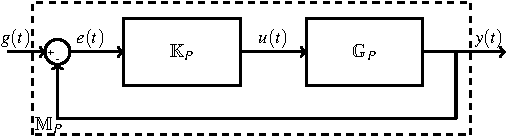
\includegraphics[scale=0.8]{KpGp.pdf}
	\caption{Feedback controller designed using VRFT}
	\end{figure}
\end{enumerate}
	To satisfy plant constraints, the reference signal $g(t)$ is generated using an MPC controller in an outer loop. The objective of the MPC controller is to make the output signal $y(t)$ track the reference $r(t)$, while satisfying constraints on the plant output $y(t)$ and input $u(t)$. This is achieved by considering the closed-loop plant model $\mathbb{M}_P$ for the state propagation equation, and an augmented model with $[y(t),u(t)]$ as the output equation. This augmented state-space model is called $\mathbb{M}'_P$.
	\begin{equation*}
	\begin{matrix}
	\zeta(t+1) = A_\zeta\zeta(t) + B_\zeta g(t)\\
	\begin{bmatrix}y(t)\\u(t)\end{bmatrix} = C_\zeta\zeta(t) + D_\zeta g(t)
	\end{matrix}
	\end{equation*}
	\\
	The optimization problem solved by the MPC at each time step $t$ for a horizon of $N_P$ timesteps is shown in \eqref{MPC}.
	\begin{equation}
	\begin{aligned}
	& \underset{\{g(t+k)\}_{k=1}^{N_P}}{\text{min}}
	& & Q_y\mathlarger{\sum\limits_{k=1}^{N_P}}(y(t+k|t)-r(t+k))^2 + Q_{\epsilon}\epsilon^2 \\
	& \text{subject to}
	& & 
	\begin{matrix}
	\zeta(t+k+1) = A_\zeta\zeta(t+k) + B_\zeta g(t+k)\\
	\begin{bmatrix}y(t+k)\\u(t+k)\end{bmatrix} = C_\zeta\zeta(t+k) + \begin{bmatrix}0\\D_\zeta\end{bmatrix}g(t+k)\\
	y_{min}-V_y\epsilon \leq y(t+k) \leq y_{max}+V_y\epsilon \\
	u_{min}-V_u\epsilon \leq u(t+k) \leq u_{max}+V_u\epsilon \\
	\zeta(t|t) = \zeta(t)
	\end{matrix}
	\end{aligned}
	\label{MPC}
	\end{equation}
	The quantities $V_y$ and $V_u$ in the MPC formulation are used as soft constraints to avoid infeasibility of the optimization problem over successive iterations, since the reference model $\mathbb{M}'_P$ might not accurately capture the dynamics of the closed loop $\mathbb{K}_P-\mathbb{G}_P$. This implies that constraint satisfaction is not guaranteed by the proposed formulation. 
	
	\subsection{Robust reference governor}
	The robust reference governer is a signal regulator which alters the command input such that the plant constraints are robustly satisfied. A schematic of the heirarchical control system with the additional robust reference governor is shown in Fig.\ref{fullloop}. 
	\begin{figure}[h]
		\vspace{-3pt}
		\hspace{10pt}
		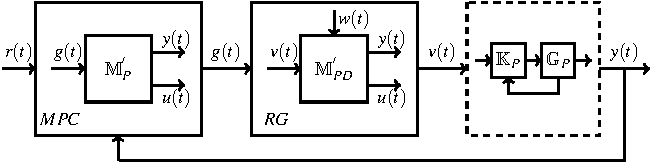
\includegraphics[scale = 0.8]{withRG.pdf}
		\caption{Schematic of the robust control system}
		\label{fullloop}
	\end{figure} 
	
	In order to achieve robustness, the reference governer $RG$ uses the model $\mathbb{M}'_{PD}$. $\mathbb{M}'_{PD}$ is a model of the closed loop performance of $\mathbb{K}_P$-$\mathbb{G}_P$, which is obtained by appending disturbance information over the model $\mathbb{M}'_{P}$. Identification of this model and corresponding bounds is discussed in Sec.\ref{Contribution}. The state space form of this model is written as:
	\begin{equation}
	\begin{matrix}
	\gamma(t+1) = A_\gamma\gamma(t) + B^v_\gamma v(t) + B^n_\gamma n(t) \vspace{2pt}\\
	\begin{bmatrix}y(t)\\u(t)\end{bmatrix} = C_\gamma\gamma(t) + D^v_\gamma v(t) + D^n_\gamma n(t)
	\end{matrix}
	\label{M_PD}
	\end{equation}
	The model has a deterministic input $v(t)$ and a disturbance input $n(t)$, which captures the effect of model uncertainties on system output. It is assumed that the disturbance input lies in a bounded set $\mathcal{N}_{\infty}$.
	The columns of matrices $B_\gamma$ and $D_\gamma$ are separated for ease of notation. The outputs of the system are called $y_{\gamma}(t)=[y(t) \hspace{2pt} u(t)]^T$. The constraints on these outputs are written as: 
	\begin{equation*}
	\begin{matrix}
	\begin{matrix}
	y_{min} \leq y(t) \leq y_{max} \\
	u_{min} \leq u(t) \leq u_{max}
	\end{matrix} & \bigg{\}} & Hy_{\gamma}(t) \leq h
	\end{matrix}
	\end{equation*}
	At each time instant $t$, the reference governer solves the quadratic program:
	\begin{equation}
	\begin{aligned}
	& \underset{v}{\text{min}}
	& & \cfrac{1}{2}\norm{v-g(t)}_2^2 \\
	& \text{subject to}
	& & 
	(x,v) \in \mathbb{O}_{\infty}
	\end{aligned}
	\label{RGprob}
	\end{equation}
	where the set $\mathbb{O}_{\infty}$ is defined as:
	\begin{equation*}
	\mathbb{O}_{\infty} = \{(x,v): x = \gamma(t), \hspace{2pt} Hy_{\gamma}(\tau) \leq h \hspace{5pt} \forall \tau \geq t \} \\ 
	\end{equation*}
	This is called a maximal output admissible set.
	It is set of feasible values for $v$ for the current observed state $x=\gamma(t)$ such that if a constant input signal $v(\tau \geq t)=v$ is applied, the system output constraints $Hy_{\gamma}(\tau \geq t) \leq h$ remain satisfied for all $\tau$.
	At a time instant $\tau \geq t$, the system output $y_{\gamma}(\tau)$ for input signal $v(\tau \geq t)=v$ can be written as:
	\begin{equation*}
	\hspace{-30pt}
	\begin{aligned}
	\begin{matrix}
	y_{\gamma}(\tau) = C_{\gamma}A_{\gamma}^{\tau - t}\gamma(t) + \bigg( C_{\gamma}\sum\limits_{k=1}^{\tau - t}A_{\gamma}^{k-1}B^v_{\gamma} + D_{\gamma}^v \bigg)v + \vspace{5pt}\\  \hspace{110pt} C_{\gamma}\sum\limits_{k=1}^{\tau - t}A_{\gamma}^{k-1}B^n_{\gamma}n(\tau-k) + D_{\gamma}^n n(\tau)
	\end{matrix}
	\end{aligned}
	\end{equation*} \\
	For a particular future time instant $\tau$, the set $\mathbb{O}_{\tau}$ is given by:
	\begin{equation*}
	\begin{matrix}
	\mathbb{O}_{\tau} = \{(x,v): x = \gamma(t), \hspace{5pt} \tilde{H}(\tau)v \leq \tilde{h}(\tau)\} \vspace{5pt}\\
	\text{where } \hspace{5pt} \tilde{H}(\tau) = H\bigg( C_{\gamma}\sum\limits_{k=1}^{\tau - t}A_{\gamma}^{k-1}B^v_{\gamma} + D_{\gamma}^v \bigg) \vspace{5pt} \\ \hspace{10pt}
	\tilde{h}(\tau) = h - HC_{\gamma}A_{\gamma}^{\tau - t}\gamma(t) - f^n(\tau) \vspace{5pt}
	\end{matrix} 
	\end{equation*}
	Each element $f^n_i(\tau)$ of the column vector $f^n(\tau)$ is calculated by solving the linear program:
	\begin{equation}
	f_i^n(\tau) = \underset{\{n(k)\}_{t}^{\tau}\in \mathcal{N}_{\infty}}{\text{max}} H\bigg(C_{\gamma}\sum\limits_{k=1}^{\tau - t}A_{\gamma}^{k-1}B^n_{\gamma}n(\tau-k) + D_{\gamma}^n n(\tau)\bigg)_i
	\label{RG_offline}
	\end{equation}
	Subscript $i$ in the above problem indicates that row $i$ of the matrix is used in the linear program to calculate the corresponding $n(k)$ sequence. According to the theory of maximal output admissible sets for linear systems as discussed in \cite{83532}, the set $\mathbb{O}_{\infty} = \mathbb{O}_{\tau \to \infty}$ is reached at a finite value $\tau_c$. In the current setting, this happens when elements of $f^n(\tau)$ converge to a constant value. Since the linear problem to be solved for $f_i^n(\tau)$ does not depend on the state at current time instant $t$, it can be solved offline for increasing values of $\tau$ after setting $t=1$. When convergence is observed at time $\tau_c$, the value $f^n(\tau_c)$ is stored. This results in  problem \eqref{RGprob} being reformulated as:
	\begin{equation}
	\begin{aligned}
	& \underset{v}{\text{min}}
	& & \cfrac{1}{2}\norm{v-g(t)}_2^2 \\
	& \text{subject to}
	& & 
	\tilde{H}(\tau_c)v \leq \tilde{h}(\tau_c)
	\end{aligned}
	\label{RGprob_simple}
	\end{equation}
	It must be noted that the value $\tilde{h}(\tau_c)$ depends on the current observed state $\gamma(t)$. Thus, at each time instant, the reference governer reads the current state $\gamma(t)$, reference input $g(t)$, and calculates a new reference $v$ which robustly satisfies output constraints on the system.
	\section{Disturbance sensor}
	\label{Contribution}
	This section discusses the development of the model $\mathbb{M}'_{PD}$, which is used by the robust reference governor to generate the signal $v(t)$. First, the overall model is presented. Then, a novel technique is introduced to quantify uncertainty bounds on the model obtained from ARX estimation.
	\subsection{Appended closed-loop model}
	In order to improve prediction of closed loop performance, a disturbance sensor $\mathbb{D}$ is designed. The disturbance sensor is a dynamical system whose output is the discrepancy between output of the actual closed loop system  $\mathbb{K}_P$-$\mathbb{G}_P$ and reference closed loop system $\mathbb{M}_P$. The system consists of a deterministic part and a stochastic part, as seen in Fig. \ref{Appended}.
	\begin{figure}[h!]
		\hspace{35pt}
		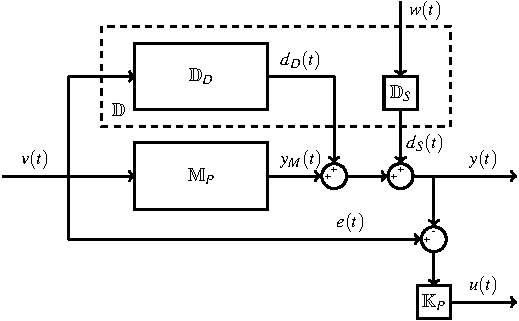
\includegraphics[scale = 0.7]{Mp-D-E.pdf}
		\caption{Reference model appended with disturbance sensor.}
		\label{Appended}
	\end{figure}
	\vspace{-5pt} \\
	Since this model represents closed loop behavior of the system, new closed loop measurements are required to estimate the parameters of the disturbance sensor. These are obtained by performing experiments with excitation signals $\hat{v}(t)$ on the reference closed loop model $\mathbb{M}_P$ and the closed loop plant $\mathbb{K}_P-\mathbb{G}_{P}$, and measuring the outputs $\hat{y}_M(t)$ and $\hat{y}(t)$ respectively. The signals are captured in the data set $\hat{D}_{N}=\{\hat{v}(t),\hat{y}_M(t),\hat{y}(t);t\in{1,...,N}\}$.
	The disturbance sensor $\mathbb{D}$ is parameterized as $A_D(q^{-1})y_D(t) = B_D(q^{-1})v(t)+w(t)$, where 
	\begin{equation*}
	\begin{matrix}
	y_D(t) = y(t) - y_M(t) = d_D(t)+d_S(t) \\ 
	A_D(q^{-1}) = 1+\mathlarger{\sum\limits_{i=1}^{n_{a_D}}}a_i^Dq^{-i}\\
	B_D(q^{-1}) = \mathlarger{\sum\limits_{i=1}^{n_{b_D}}}b_i^Dq^{-i}
	\end{matrix}  
	\end{equation*}
	\iffalse
	\begin{table*}[ht]
		\begin{center} 
			\begin{adjustbox}{width=0.9\textwidth,center=\textwidth}
				\begin{tabular}[h]{ c|c }
				\centering
				\setlength{\tabcolsep}{0.1em}
				$
				\begin{matrix}
				\underset{X_{min}}{\text{max}}
				& w^N_{min} \\
				\text{subject to}
				& 
				d_S(k) = -\mathlarger{\sum\limits_{i=1}^{n_{a_D}}}a_i^Dd_S(k-i) + w(k), k={1:N}\\
				& d_{S,min} \leq d_S(k) \leq d_{S,min}, k={1:N-1} \vspace{4pt}\\
				& w^N_{min} \leq w(k), k={1:N} \vspace{3pt}\\
				& d_S(N) \leq d_{S,min} 
				\end{matrix} 
				$
				&
				$
				\begin{matrix}
				\underset{X_{max}}{\text{min}}
				& w^N_{max} \\
				\text{subject to}
				&
				d_S(k) = -\mathlarger{\sum\limits_{i=1}^{n_{a_D}}}a_i^Dd_S(k-i) + w(k), k={1:N}\\
				& d_{S,min} \leq d_S(k) \leq d_{S,min}, k={1:N-1} \vspace{4pt}\\
				& w(k) \leq w^N_{max}, k={1:N} \vspace{3pt}\\
				& d_S(N) \geq d_{S,max} \\
				\end{matrix}
				$
				\vspace{10pt}\\
				$
				\text{where } X_{min} = 
				\begin{Bmatrix}
				\{d_S(-n_{a_D}+1),...,d_S(N)\},\\
				\{w(1),...,w(N)\},\vspace{0.001cm}\\
				w^N_{min}
				\end{Bmatrix}
				$
				&
				$
				\text{where } X_{max} = 
				\begin{Bmatrix}
				\{d_S(-n_{a_D}+1),...,d_S(N)\},\\
				\{w(1),...,w(N)\},\vspace{0.001cm}\\
				w^N_{max}
				\end{Bmatrix}
				$
			\end{tabular}}
			\end{adjustbox}
		\end{center}
		\label{w_calculation}
		\caption{Linear programs solved to calculate the set $\mathcal{W}_{\infty}$}
	\end{table*}
	\fi
	
	Using standard ARX identification, the coefficients $a_i^D$ and $b_i^D$ are estimated by solving the optimization problem
	\begin{equation}
	\begin{aligned}
	& \underset{a_i^D,b_i^D}{\text{min}}
	& & \frac{1}{N}\mathlarger{\sum\limits_{t=1}^N}\mathlarger{\mathlarger{|}}A_D(q^{-1})(\hat{y}(t)-\hat{y}_M(t))-B_K(q^{-1})(\hat{v}(t))\mathlarger{\mathlarger{|}}^2 \\
	\end{aligned}
	\label{DSensor}
	\end{equation}
	The disturbance sensor is then split into two parts, deterministic and stochastic. The deterministic part $\mathbb{D}_D$ takes in the reference signal $v(t)$ as an input, and the stochastic part $\mathbb{D}_S$ takes in the exogenous disturbance $w(t)$. The I/O behavior of these parts are separately written as 
	\begin{equation*}
	\begin{matrix}
	d_D(t) = \cfrac{B_D(q^{-1})}{A_D(q^{-1})}v(t) = \mathbb{D}_D v(t) \vspace{4pt} \\  
	d_S(t) = \cfrac{1}{A_D(q^{-1})}w(t) = \mathbb{D}_S w(t)
	\end{matrix}
	\end{equation*}
	The overall appended model shown is Fig.\ref{Appended} can be seen as a 2-input 2-output system $\mathbb{M}'_{PD}$, described as
	\begin{equation}
	\begin{bmatrix}
	y(t) \\ u(t)
	\end{bmatrix} = 
	\begin{bmatrix} 
	\mathbb{M}_P+\mathbb{D}_D & \mathbb{D}_S \\
	\mathbb{K}_P(I-(\mathbb{M}_P+\mathbb{D}_D)) &  -\mathbb{K}_P\mathbb{D}_S
	\end{bmatrix}
	\begin{bmatrix}
	v(t) \\ w(t)
	\end{bmatrix}
	\label{TF_w}
	\end{equation}
	Alternatively, it can also be seen a system with $d_S(t)$ acting as measurement noise on the output $y(t)$. The model corresponding to this view-point is:
	\begin{equation}
	\begin{bmatrix}
	y(t) \\ u(t)
	\end{bmatrix} = 
	\begin{bmatrix} 
	\mathbb{M}_P+\mathbb{D}_D & I \\
	\mathbb{K}_P(I-(\mathbb{M}_P+\mathbb{D}_D)) &  -\mathbb{K}_P
	\end{bmatrix}
	\begin{bmatrix}
	v(t) \\ d_S(t)
	\end{bmatrix}
	\label{TF_d}
	\end{equation} 
	Note that the dependence of the model on time shift operator $q^{-1}$ is not shown for ease of notation. Both $w(t)$ and $d_S(t)$ can be seen as exogenous disturbance signals, which cause model uncertainty. Hence, the state space equivalents of either of these models can be used in a robust reference governor, by replacing $n(t)$ in \eqref{M_PD} with $w(t)$ if model \eqref{TF_w} is used, and with $d_S(t)$ if \eqref{TF_d} is used. \\
	If the model described in \eqref{TF_d} is considered for robust reference governor design, the bounds on $d_S(t)$ can be estimated directly from the prediction errors obtained during ARX identification performed in \eqref{DSensor}. These bounds are used to build the set $\mathcal{D}_{\infty}$, the definition of which is formalized in the next subsection. Within the reference governor, the disturbance set $\mathcal{N}_{\infty}$ is set equal to $\mathcal{D}_{\infty}$.
.	In case of the model described in \eqref{TF_w}, the calculation of bounds on $w(t)$ is not as straightforward. 
	The following subsection discusses a technique to calculate upper and lower bounds $w_{min}$ and $w_{max}$ on the disturbance signal $w(t)$, which build the set $\mathcal{W}_{\infty}$. In the reference governor, $\mathcal{N}_{\infty}$ is then set equal to $\mathcal{W}_{\infty}$
	\subsection{Calculation of exogenous disturbance set}
	\label{Noise}
	A realization of the discrepancy $d_S(t)$ between desired output $y(t)$ and deterministic output $y_M(t)+d_D(t)$ can be calculated from the data set $\hat{D}_{N}$ as 
	\begin{equation*}
	\hat{d}_S(t) = \hat{y}(t)-\hat{y}_M(t)-\cfrac{B_D(q^{-1})}{A_D(q^{-1})} \hat{v}(t) 
	\end{equation*}
	The maximum and minimum values of this discrepancy are labeled $\hat{d}_{S,max}$ and $\hat{d}_{S,min}$ respectively. If the ARX identification results in a stable deterministic disturbance sensor $\mathbb{D}_D$, the values $\hat{d}_{S,max}$ and $\hat{d}_{S,min}$ are finite. Further, if infinite closed loop data $\hat{D}_{\infty}$ is collected for ARX identification, the bounds on discrepancy are equal to the actual bounds $d_{S,max}$ and $d_{S,min}$. The set of sequences $d_S(t)$ satisfying these bounds are indicated as lying in a set $\mathcal{D}_{\infty}$, defined as 
	\begin{equation*}
	\mathcal{D}_{\infty} = \{d_S(t): d_{S,min} \leq d_S(t) \leq d_{S,max} \hspace{5pt} \forall t \in (-\infty,\infty) \}
	\end{equation*}
	 From these bounds, we attempt to calculate the set $\mathcal{W}_{\infty}$ defined as
	\begin{equation*}
	\mathcal{W}_{\infty} = \begin{Bmatrix} w(t): \forall t \in (-\infty,\infty), \begin{matrix}
	w_{min}\leq w(t)\leq w_{max} \\ 
	\mathbb{D}_S w(t) \in \mathcal{D}_{\infty} \\
	\end{matrix} 
	\end{Bmatrix}
	\end{equation*}  
	This is the set of all $w(t)$ sequences such that the steady-state output signal of $\mathbb{D}_S$ corresponding to any $w(t)\in \mathcal{W}_{\infty}$  lies within $\mathcal{D}_{\infty}$. It must be noted that the converse is not implied. That is, it does not mean that there cannot exist a noise sequence $w(t)$ not belonging to $\mathcal{W}_{\infty}$ but producing a corresponding output sequence belonging to $\mathcal{D}_{\infty}$.
	\begin{equation*}
	\begin{matrix}
	\hspace{-40pt}\forall w(t) \in \mathcal{W}_{\infty}  : \mathbb{D}_S w(t) \in \mathcal{D}_{\infty} \\
	\hspace{40pt}\notimplies \nexists  w(t) \notin \mathcal{W}_{\infty} : \mathbb{D}_S w(t) \in \mathcal{D}_{\infty}
	\end{matrix}
	\end{equation*}
	This means that the bounds on residuals of the ARX identification \eqref{DSensor}, that can be obtained by inverting the (invertible) model $\mathbb{D}_S$, are not necessarily $w_{min}$ and $w_{max}$. 
		
	To calculate the bounds $w_{min}$ and $w_{max}$, first, the optimization problems shown in \eqref{bound_problem} are solved for increasing lengths of time horizon $N$.
	\begin{equation}
	\begin{matrix}
	\begin{matrix}
	\underset{X_{j}}{\text{min}}
	& \bar{w}_j(N) \\
	\text{subject to}
	& 
	d_S(k) = -\mathlarger{\sum\limits_{i=1}^{n_{a_D}}}a_i^Dd_S(k-i) + w(k), k={1:N}\\
	&  d_{S,min} \leq d_S(k) \leq d_{S,max}, \hspace{5pt} k={1:N-1} \vspace{4pt}\\
	&  -\bar{w}_j(N) \leq w(k) \leq \bar{w}_j(N), \hspace{5pt} k={1:N} \vspace{3pt}\\
	&  d_S(N) \in D_j 
	\end{matrix}
	\vspace{10pt} \\
	\text{where } X_j = 
	\begin{Bmatrix}
	\{d_S(-n_{a_D}+1),...,d_S(N)\},\\
	\{w(1),...,w(N)\},\vspace{0.001cm}\\
	\bar{w}_j(N)
	\end{Bmatrix}, j=\{1,2\}
	\vspace{5pt}\\
	\begin{matrix}
	D_1 = \{d:d \leq d_{S,min}\}\\
	D_2 = \{d:d \geq d_{S,max}\}
	\end{matrix}
	\end{matrix}
	\label{bound_problem}
	\end{equation}
	
	These equations solve for a sequence of inputs $\{w(k), k={1:N}\}$ such that the sequence of corresponding outputs at all instances except at time $N$ lie within $\mathcal{D}_{\infty}$. This means that the chosen input sequence $w(k)$ should drive $d_S(N)$ out of $\mathcal{D}_{\infty}$ into $D_j$. The initial conditions on $d_S(k)$ are left free to be chosen by the problem, but are constrained to lie within $\mathcal{D}_{\infty}$.
	The solutions $\bar{w}_j(N)$ are collected, and the set $\mathcal{W}_{\infty}$ is calculated using \eqref{maxmin}. It is noted that the noise is assumed to be zero-mean. This can be rectified easily by letting the lower and upper bounds on $w(k)$ in \eqref{bound_problem} be composed of different optimization variables.
	\begin{equation}
		\begin{matrix}
		w_{max} = {\text{max }}\{\underset{N}{\text{max }} \bar{w}_1(N),\underset{N}{\text{max }}\bar{w}_2(N)\} \\
		w_{min} = {\text{min }}\{\underset{N}{\text{min }}-\bar{w}_1(N),\underset{N}{\text{min }}-\bar{w}_2(N)\} \\
		\end{matrix}
		\label{maxmin}
	\end{equation}
	At lower values of $N$, there can exist an initial sequence $\{d_S(-n_{a_D}+1),..,d_S(1)\}$ that drives $d_S(N)$ into $D_j$ with very low control effort. At higher values of $N$, the effect of initial condition wears off, and a higher value of control effort is required to violate $\mathcal{D}_{\infty}$. Hence, solving \eqref{maxmin} gives the values of $w_{min}$ and $w_{max}$, that are the minimum and maximum values of the disturbance signal $w(t)$ such that the steady state values of $d_S(t)$ lie within $\mathcal{D}_{\infty}$.  
	%\begin{figure}[h!]
		%\begin{center}
			%\hspace{20pt}
			%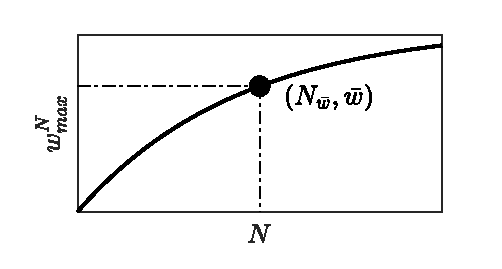
\includegraphics[scale = 0.85]{explain.eps}
			%\hspace{20pt}
			%\caption{An illustration of the bounds for the case of %$w_{max}$ calculation. Any sequence %$||w(t)||_{\infty}=\bar{w}$ can drive $d_S(t)\geq %d_{S,max}$ only after $k \geq N_{\bar{w}}$ of %application. We want to find the value of %$w^N_{max}=\bar{w}$ such that $N=N_{\bar{w}} \to \infty$. %This is $w_{max}$. The analogous opposite applies to the %calculation of $w_{min}$.   }
	%		\label{explanation}
	%	\end{center}
	%\end{figure} 
	%Any sequence $\{w(k)>w^N_{min},k=1:N\}$ will not drive $d_S(k \geq N)$ to the bound $d_{S,min}$. Similarly, $\{w(k)<w^N_{max},k=1:N\}$ will not drive $d_S(k \geq N)$ to the bound $d_{S,max}$. Hence, in order to explain the whole set $\mathcal{D}_{\infty}$, we need to find the lowest possible value of $w^N_{min}$ and the highest possible value of $w^N_{max}$ such that $d_S(k)$ is driven to its bounds in finite time $k$. This is achieved by increasing the value of $N$, which would require lower and higher values of $w(k)$ to make $d_S(N)$ reach $d_{S,min}$ and $d_{S,max}$ respectively. This leads to $w^N_{min}$ and $w^N_{max}$ asymptotically reaching their true values $w_{min}$ and $w_{max}$ as $N$ increases, thus making the set $\mathcal{W}_{\infty}$ completely explain the set $\mathcal{D}_{\infty}$.
	 %It is noted that the presented method provides a methodology to quantify uncertainty in any general ARX identified model.%
	 \\
	We now have a closed-loop model with disturbance bound information, and hence are ready to use it in a robust reference governor.
	\section{Case study}
	Numerical simulations are performed on a servo motor control problem, implementing the complete control scheme presented in Fig.\ref{fullloop}. The sampling time is $Ts = 1 ms$. Reference governors are implemented for closed loop models corresponding to both \eqref{TF_w} and \eqref{TF_d}. It is shown that using model \eqref{TF_w} results is superior performance, and hence performing an additional step to calculate $w_{min}$ and $w_{max}$ is justified.
	Both the case studies are implemented using MATLAB R2017b, with optimization problems occasionally implemented using YALMIP \cite{Lofberg2004}.
	\label{Case studies}
	%%%%%%%%%%%%%%%%%%%%%%%%%%%%%%%%%%%%%%%%%%%%%%%%%%%%%%
	\iffalse
	\subsection{Noise input bound}
	Consider a MISO system with inputs $\{u(t),w(t)\}$ and output $x(t)$, described by:
	\begin{equation*}
	\begin{matrix}
	u(t+1) = 0.995u(t)+1 \\
	x(t+1) = 0.05x(t)+u(t)+w(t) \\
	u(1) = 0, \hspace{5pt} x(1) = 0
	\end{matrix}
	\end{equation*}
	The input $u(t)$ is deterministic and $w(t)$ is the disturbance. An approximate ARX model of the system is calculated as $A(q^{-1})\tilde{x}(t) = B(q^{-1})u(t)+w(t)$ after performing experiments on the system and collecting data. It is identified with $A(q^{-1})$ and $B(q^{-1})$ having two and one free parameter each. Following this, the methodology discussed in Sec.\ref{Noise} is used to calculate bounds on $w(t)$.
	\\
	First, the signal $d_S(t)=x(t) - (B(q^{-1})/A(q^{-1}))u(t)$ is extracted from the experimental data, and $\mathcal{D}_{\infty}$ is constructed. For increasing values of $N$, sequences $\{w(k),k=1:N\}$ and corresponding $\{d_S(k),k=1:N\}$ are calculated by solving the optimization problems in \eqref{bound_problem}. The bounds $-\bar{w}_j(N)$ and $\bar{w}_j(N)$ on the input sequences are shown in Fig.\ref{bounds}.
	The largest region where $-\bar{w}_j(N) \leq w(k) \leq -\bar{w}_j(N)$ is satisfied, is $\mathcal{W}_{\infty}$. 
		\begin{figure}[h!]
			\hspace{30pt}
			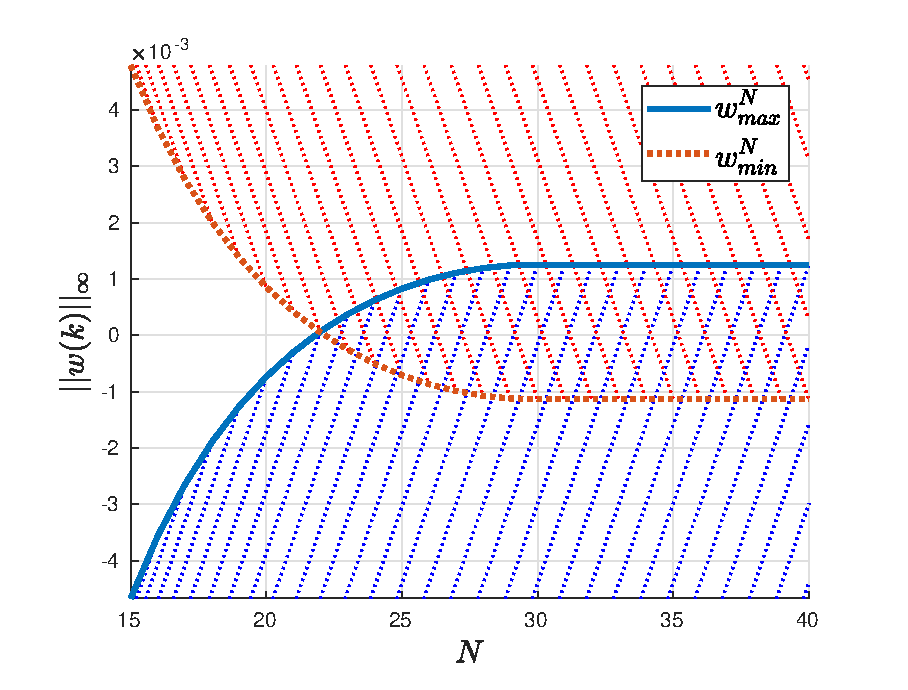
\includegraphics[scale = 0.60]{bounds.eps}
			\caption{Convergence of bounds to $w_{min}$ and $w_{max}$, with zero mean noise assumption.}
			\label{bounds}
		\end{figure} \vspace{-5pt}\\
	To verify the obtained bounds, the system identified through ARX identification is simulated with deterministic inputs $u(t)$, and a range of disturbance inputs $w(t)$ sampled from $\mathcal{W}_{\infty}$. The simulation results are seen in Fig.\ref{simulation}. It can be seen that output of the ARX model simulated with noise inputs $w(t)$ covers the measurement range, and avoids conservatism. This is an indicator that the set $\mathcal{W}_{\infty}$ is valid.
	\begin{figure}[h]
		\hspace{22pt}
		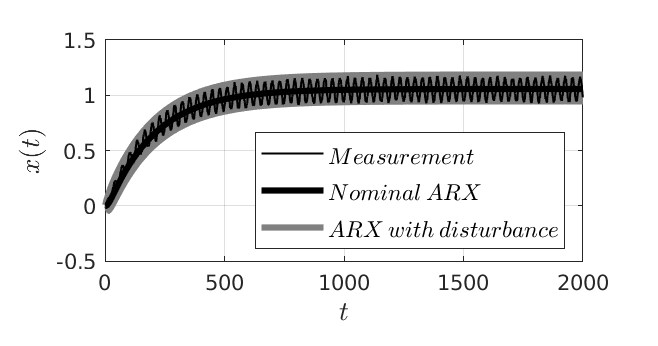
\includegraphics[scale = 0.70]{simulation.eps}
		\caption{Comparison of ARX model performance with constant $w(t)=0$(nominal) and $w(t)\in \mathcal{W}_{\infty}$. The appended disturbance model gives bounded output $x(t)$ without being conservative.}
		\label{simulation}
	\end{figure} 
	The simulation of ARX model with disturbance requires an initial condition on the disturbance model $\mathbb{D}_S$. In the current example, it is set to $0$. Since the actual initial condition of $\mathbb{D}_S$ might not be $0$, one might face problems with the model not covering the whole range of $\mathcal{D}_{\infty}$ during the transient period. To correct this, a state estimator could be used which rectifies the effect of initial state discrepancy, thus covering the noise effects even during transients.
	\fi
	%%%%%%%%%%%%%%%%%%%%%%%%%%%%%%%%%%%%%%%%%%%%%%%%%%%%%%
	\subsection{Data driven MPC with robust reference governer}
	The plant consisting of a servo positioning system is controlled using the scheme shown in Fig.\ref{fullloop}. The plant dynamics are modeled with the following non-linear state space equations:
	\begin{equation*}
	\begin{matrix}
	\begin{bmatrix}
	\dot{\theta}(t) \vspace{12pt} \\
	\dot{\omega}(t) \vspace{12pt} \\
	\dot{i}(t)
	\end{bmatrix} = 
	\begin{bmatrix}
	\omega(t) \vspace{3pt}\\
	\cfrac{-mgl}{J}\hspace{1pt}sin\theta(t)-\cfrac{b}{J}\hspace{1pt}\omega(t) + \cfrac{K_m}{J}\hspace{1pt}i(t) \\  
	\cfrac{-K_m}{L}\hspace{1pt}\omega(t)-\cfrac{R}{L}\hspace{1pt}i(t) + \cfrac{1}{L}\hspace{1pt}u(t)
	\end{bmatrix} \vspace{10pt}\\
	y(t) = \begin{bmatrix} 1 & 0 & 0 \end{bmatrix} 
	\begin{bmatrix} \theta(t) \\ \omega(t) \\ i(t) \end{bmatrix} 
	\end{matrix}
	\end{equation*}
	
	\begin{table}[h!]
		\hspace{30pt}
		\begin{tabular}{||c|c|c||} 
			\hline
			Symbol & Parameter & Value\\ [0.5ex] 
			\hline\hline
			$R$ & Motor resistance & $5\Omega$ \\ 
			%\hline
			$L$ & Motor inductance & $5.10^{-3}$H \\
			%\hline
			$K_m$ & Motor torque constant & $0.0847$Nm/A \\
			%\hline
			$J$ & Complete disk inertia & $5.10^{-5}$Nm$^2$ \\
			%\hline
			$b$ & Friction coefficient & $3.10^{-3}$Nms/rad \\
			%\hline
			$m$ & Additional mass & $3$Kg \\
			%\hline
			$l$ & Mass offset & $2$m \\
			\hline
		\end{tabular}
		\caption{Physical parameters of servo motor system}
		\label{Simparam}
	\end{table}
	The states of the system $\theta(t)$,$\omega(t)$ and $i(t)$ are angle $[rad]$ and rotational velocity $[rad/s]$ of the servo motor, and armature current $[A]$ respectively. The input $u(t)$ is the voltage $[V]$ applied across the motor, and output $y(t)$ is the rotational angle. 
	A VRFT methodology is used to design a stabilizing PD controller, which provides a voltage input $u(t)$ to make the rotational angle $y(t)$ track a reference signal $g(t)$. To this end, experiments are conducted with a low-pass filtered white noise signal $u(t)$ with a standard deviation of $10$V. The output angle $y(t)$ is recorded and the dataset $\mathbb{D}_N$ is obtained. A slow reference closed loop model $\mathbb{M}_P$ is chosen, given by:
	\begin{equation*}
	\begin{matrix}
	x_M(t+1) = 0.99x_M(t) + 0.01g(t)\\
	y_M(t) = x_M(t)
	\end{matrix}
	\end{equation*}
	The PD inner-loop controller $\mathbb{K}_P$ is parameterized as:
	\begin{equation*}
	u(t) = K_pe(t) + K_d\cfrac{e(t)-e(t-1)}{Ts}
	\end{equation*} 
	Solving the optimization problem \eqref{VRFT_problem}, the parameters 
	$K_p$ and $K_d$ are calculated using the dataset $D_N$. The controller is placed in the inner loop within the hierarchical control architecture.
	After VRFT synthesis, an outer MPC is designed using the formulation in \eqref{MPC}, to provide a reference signal $g(t)$. The output $y(t)$ is constrained to lie between $0$ rad and $4$ rad, and the voltage input $u(t)$ between $-3.5$ V and $3.5$ V. An MPC horizon of $N_P=10$ timesteps is chosen, and weights are $Q_y=1$ and $Q_{\epsilon}=1$. \\
	Towards formulating the robust reference governor, the disturbance sensor discussed in Sec.\ref{Contribution} is developed. First, the dataset $\hat{D}_N$ is built by performing closed loop experiments with input signal $\hat{v}(t)$ of standard deviation $10$ rad. Then, a linear model for $\mathbb{D}$ parameterized by $n_{a_D} = 4$ and $n_{b_D} = 3$ is identified by solving \eqref{DSensor}. Two equivalent models of the appended system, corresponding to \eqref{TF_w} and \eqref{TF_d}, are developed.  \\ 
	\indent For the model corresponding to \eqref{TF_w}, the disturbance sensor is split into two parts, $\mathbb{D}_D$ and $\mathbb{D}_S$, with inputs $v(t)$ and $w(t)$ respectively. Bounds on the exogenous disturbance $w(t)$ for a horizon $N$ are calculated by solving the linear problems \eqref{bound_problem}. The evolution of these bounds with increasing values of horizon $N$ is plotted in Fig.\ref{bounds_RG}.  The values $w_{min}$ and $w_{max}$ are obtained by solving \eqref{maxmin}.
	\begin{figure}[h]
		\hspace{30pt}
		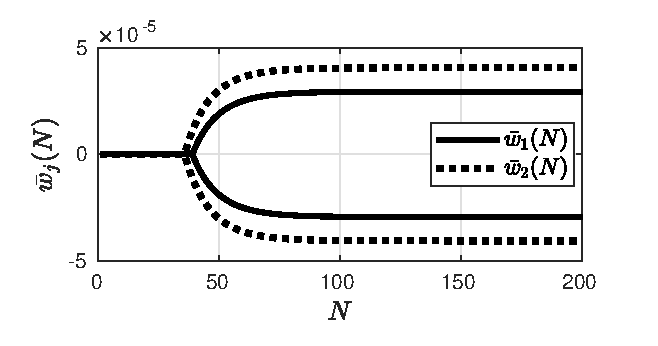
\includegraphics[scale = 0.6]{bounds_RG.eps}
		\caption{Convergence of bounds on $w(t)$ acting as input to the disturbance sensor $D_S$.}
		\label{bounds_RG}
	\end{figure} \\
	For the model corresponding to Eq.\eqref{TF_d}, the disturbance sensor consists of $\mathbb{D}_D$ and a direct exogenous disturbance signal $d_S(t)$. Bounds on $d_S(t)$, called $d_{S,min}$ and $d_{S,max}$, are set equal to minimum and maximum values of prediction error obtained during identification of the ARX model for $\mathbb{D}$ respectively. \vspace{5pt} \\
	These models and related disturbance bounds are used in the formulation of corresponding robust reference governors to calculate bounds on the input $v(t)$. The values of the part $f^n(\tau)$ of these bounds can be calculated offline by solving the linear programs described in \eqref{RG_offline}. These programs are usually solved till convergence, thus computing the maximal output admissible set $\mathbb{O}_{\infty}$. Such an approach, however, could result in an overly conservative bound for $v(t)$. To avoid this, the calculation of $f^n(\tau)$ is stopped after $2*N_P$ time-steps, resulting in $f^n(2*N_P*Ts)$.\\
	The corresponding output admissible set $\mathbb{O}_{2*N_P*Ts}$ is calculated at each time-instant by reading the state $\gamma(t)$, which is built with the assumption of no additional measurement noise.
	Following this,
	the quadratic program \eqref{RGprob_simple} is constructed and solved by the robust reference governor. The reference governor modifies the MPC output $g(t)$ to a constraint respecting $v(t)$. 
	Performance of the control system for all these cases is plotted in Fig.\ref{VRFT_y} and Fig.\ref{VRFT_u}.
	\begin{figure}[t]
		\hspace{-5pt}
		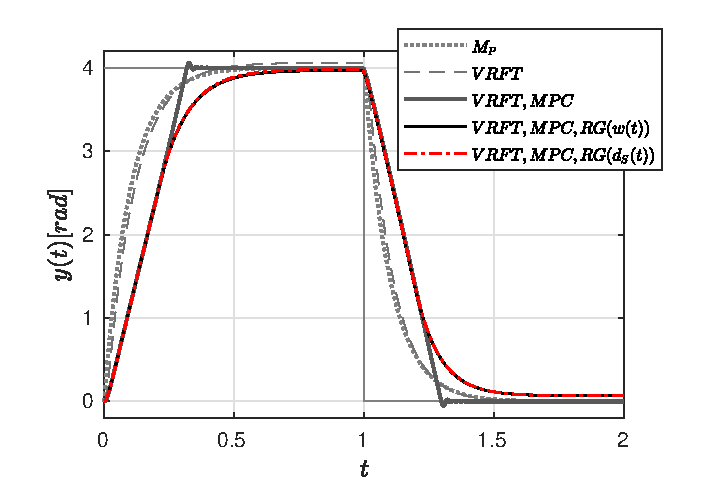
\includegraphics[scale = 0.60]{VRFT_vs_MPC.eps}
		\caption{The performance inner closed loop does not exactly match the reference model $M_P$. MPC improves the performance but results in small constraint violation. Constraint violation is robustly avoided by using a reference governor. Using \eqref{TF_d} results in a conservative performance compared to \eqref{TF_w}.  }
		\label{VRFT_y}
	\end{figure} 
	
	\begin{figure}[t]
		\hspace{-5pt}
		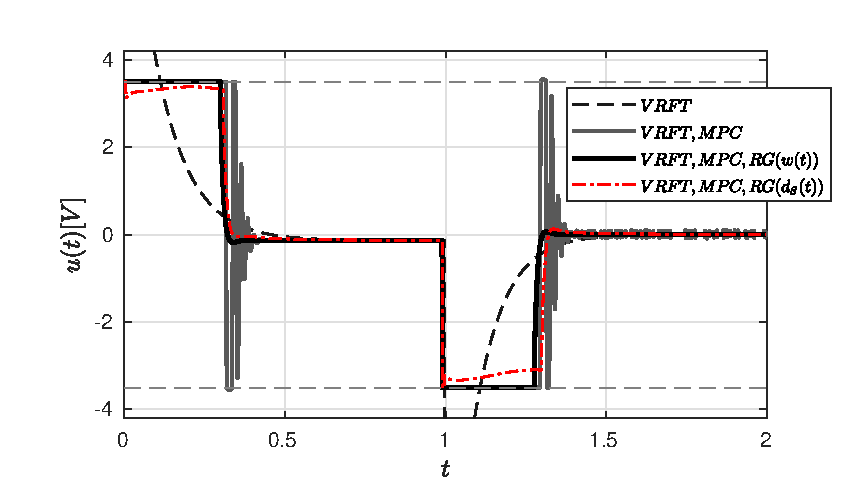
\includegraphics[scale = 0.60]{VRFT_vs_MPC_u.eps}
		\caption{Comparison of voltage input $u(t)$.}
		\label{VRFT_u}
	\end{figure} 
	It can clearly be seen that utilizing a robust reference governor to modify $g(t)$ from the MPC controller results in robust constraint satisfaction. Also, using the closed loop model corresponding to \eqref{TF_d} for robust reference governor design results in conservative performance, compared to using \eqref{TF_w}, for the same admissible set horizon $\tau = 2*N_P*Ts$. Increasing this horizon to $\tau_c$ results in comparable conservative performance from both the models. Since the calculation of bounds $w_{min}$ and $w_{max}$ is performed offline, conservativeness of the control scheme can be reduced without any additional online operation.
	
	\section{Conclusion}
	This paper builds on the hierarchical data-driven control of constrained systems, by introducing robustness with respect to constraint satisfaction. This is done by using a robust reference governor.  Uncertainty on the model utilized by the reference governor is modeled as disturbance input. 
	The major contribution of this work is the formulation of a novel technique to compute bounds on this input from ARX identification. It is seen that robust constraint satisfaction is achieved without identifying an open-loop model of the non-linear plant. Future work deals with extending the formulation to general Box-Jenkins models. Possible extensions to the control scheme includes modifications to incorporate LPV and MIMO systems.

	
                                                             
\bibliography{references}



\end{document}
